\section{Design}

In this section we will explain the design decisions that were made along the way.

\subsection{Limiting scope}

As discussed previously, there are many different types of MEV, and a long tail of exotic ways to extract value. The most obvious and most profitable way to extract value is through arbitrage. On Ethereum there exists many different kinds of exchanges, but on other chains, the selection is more scarce. In order of fees generated, the most popular DEX by far is Uniswap\cite{cryptofees}. Uniswap have multiple versions of their DEX'es deployed on the Ethereum mainnet, but only v3 is deployed on different L2's. Uniswap is also well documented, and their smart contracts emits events that make it a lot more feasible to find and organise swap data. Because of these factors, the decision was made to only look at Uniswap data from different domains in order to keep the complexity of the problem under control.

\subsection{Getting Data}
In order to detect cross domain MEV you need data from multiple domains. Transaction data for decentralised blockchains is public, but that does not mean that its readily available for average consumers. While running an ethereum node and using that to extract data from Ethereum is relatively simple on consumer hardware, if you want to run nodes for different blockchain networks, you need a lot of storage quite quickly. 

The initial idea was just to look for cross domain MEV between two domains, Mainnet Ethereum and Arbitrum, a Layer 2 (L2) scaling solution. Arbitrum \cite{arbitrum} is also powered by the Ethereum Virtual Machine (EVM) which makes building software to analyse data on the two different chains easier. We rented a server in order to sync nodes and was successful in doing so. The storage requirements for running these nodes were however greater then expected, and increasing the number of network and therefore domains we could analyse data from was too costly in this setup. 

The alternative to hosting your own nodes is using an infrastructure provider to supply the data. In our case we had previous experience with Infura, a service developed by Consensys and used by much of the Ethereum ecosystem. Infura API's allows for access to Ethereum data without running your own node, and they currently have Beta of node access from other networks. Using Infura, we were able to do 100.000 request/day to their API's for free, and extract data from Mainnet Ethereum, Arbitrum, Optimism \cite{optimism} and Polygon PoS \cite{polygonPOS}. All these networks are EVM compatible and have an instance of Uniswap v3 deployed to them.

\subsection{Smart Contract Addresses}
% Some addresses are the same across domains, some are not
The base Uniswap smart contracts are deployed on the same addresses across our chosen chains, as well as all their testnets \cite{uniswapcontracts}. This is possible because smart contract addresses are deterministic, given the smart contract byte code and the nonce of the signer. The smart contract addresses of different ERC20 are however not the same across chains. These were found manually through block explorers of the respective chains. These can then in turn be used in conjunction with the UniswapV3Factory smart contract to determine the addresses of the pools.

\subsection{Uniswap Fee Tiers}
% Different tiers on different chains, each tier own smart contract address
One of the things that were new in Uniswap v3 was the introduction of fee tiers. The idea is that some pools are more risky to provide liquidity for than others, so liquidity providers should be rewarded accordingly. For some chains, the Uniswap governance system has included an additional fee tier that is not present on all chains. When getting the addresses of the pools, that needs to be considered. The different fee tiers also result in multiple pools for each token pair.


\subsection{Swap Logs}
% Transaction emits logs, they are not stored on normal nodes, but can be reproduced. Infura has getLogs API that we can use to get logs when we know addresses and topic.
When a swap occurs in a Uniswap pool, it emits an event. Events are stored as logs by archival nodes and can be reproduced by replaying the transaction. Infura allows one to search for specific logs using their API. The Swap event consists of: \cite{swapdocs}
\begin{table}[h]
\begin{tabular}{|l|l|l|}
\hline
{\color[HTML]{1C1E21} Name}         & {\color[HTML]{1C1E21} Type}    & {\color[HTML]{1C1E21} Description}                                                              \\ \hline
{\color[HTML]{1C1E21} sender}       & {\color[HTML]{1C1E21} address} & {\color[HTML]{1C1E21} The address that initiated the swap call, and that received the callback} \\ \hline
{\color[HTML]{1C1E21} recipient}    & {\color[HTML]{1C1E21} address} & {\color[HTML]{1C1E21} The address that received the output of the swap}                         \\ \hline
{\color[HTML]{1C1E21} amount0}      & {\color[HTML]{1C1E21} int256}  & {\color[HTML]{1C1E21} The delta of the token0 balance of the pool}                              \\ \hline
{\color[HTML]{1C1E21} amount1}      & {\color[HTML]{1C1E21} int256}  & {\color[HTML]{1C1E21} The delta of the token1 balance of the pool}                              \\ \hline
{\color[HTML]{1C1E21} sqrtPriceX96} & {\color[HTML]{1C1E21} uint160} & {\color[HTML]{1C1E21} The sqrt(price) of the pool after the swap, as a Q64.96}                  \\ \hline
{\color[HTML]{1C1E21} liquidity}    & {\color[HTML]{1C1E21} uint128} & {\color[HTML]{1C1E21} The liquidity of the pool after the swap}                                 \\ \hline
{\color[HTML]{1C1E21} tick}         & {\color[HTML]{1C1E21} int24}   & {\color[HTML]{1C1E21} The log base 1.0001 of price of the pool after the swap}                  \\ \hline
\end{tabular}
\end{table}

The data we are most interested in is the sending and receiving address and the amounts of tokens that were swapped.


\subsection{Blocks}
% block times on different network, how blocks work etc etc
To limit the amount of data, we only extract from a certain period. We chose the range from the month of June as well as the first week of July of this year. This range was chosen partially to fall within the limits of how many transaction was allowed to the Infura API (100.000 pr. day) and partially to have enough space to store it comfortably. This time frame was also chosen to be as recent as possible, since the knowledge of cross domain MEV is still quite new, and we might observe more activity the later we go. 

\subsection{Connector}
% class to abstract stuff away so its easier to handle.

In order to make it seamless to extract data from multiple domains, all of the above peculiarities of extracting the data was to be organised in an abstract connector. The connectors job was to act as a simple interface that could extract data with the same methods regardless of which domain the data was coming from. 


% \subsection{Analysis}
% Something something these scripts is what all this code was meant to facilitate


\subsection{Visualisation}
% Improve this
\begin{figure}[H]
    \centering
    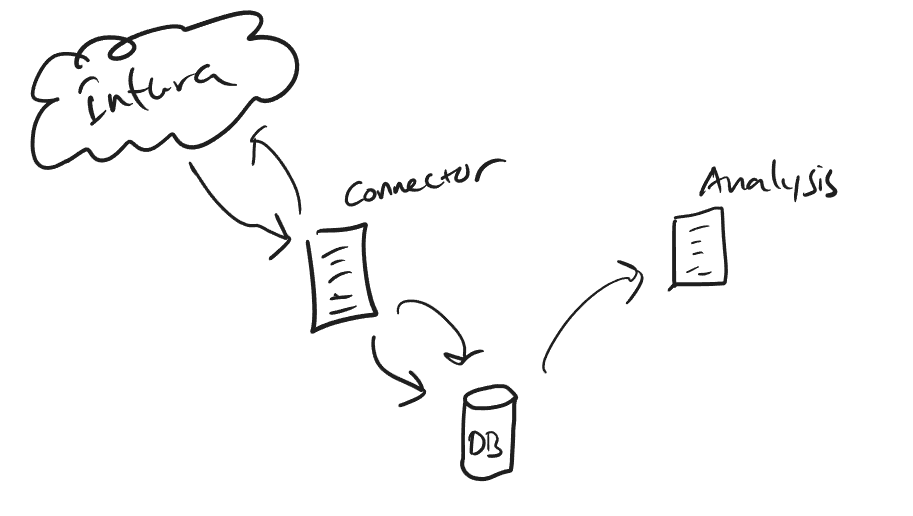
\includegraphics[width=\textwidth]{3_FIGURES/DesignImplementation/softwarewohoo.PNG}
    \caption{Diagram of System Design}
    \label{sysdiag}
\end{figure}

In short, we want to extract log event data from Infura API's in order to analyse them and find potential cross domain MEV.